55. $|y|=|x+1|\Leftrightarrow\left[\begin{array}{l} y=x+1,\\ y=-x-1.\end{array}\right.$
$$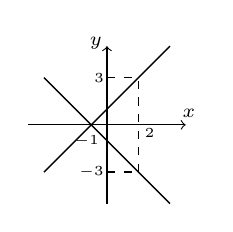
\begin{tikzpicture}[scale=0.2]
\tikzset {line01/.style={line width =0.5pt}}
\tikzset{line02/.style={line width =1pt}}
\tikzset{line03/.style={dashed,line width =0.5pt}}
%\filldraw [black] (0,0) circle (1pt);
\draw [->] (-5,0) -- (5,0);
\draw [->] (0,-5) -- (0,5);
\draw[line01] (-4,3) -- (4,-5);
\draw[line01] (-4,-3) -- (4,5);
\draw[line03] (2,-3) -- (2,3);
\draw[line03] (0,3) -- (2,3);
\draw[line03] (0,-3) -- (2,-3);
\draw (2.7,-0.5) node {\tiny $2$};
\draw (-1.3,-1) node {\tiny $-1$};
\draw (-0.5,3) node {\tiny $3$};
\draw (-1,-3) node {\tiny $-3$};
\draw (5.2,0.7) node {\scriptsize $x$};
\draw (-0.7,5.2) node {\scriptsize $y$};
\end{tikzpicture}$$
\newpage
\noindent56. Возможны три случая: точки $A$ и $B$ являются противоположными вершинами квадрата, $A$ и $B$ являются соседними вершинами и две других вершины над прямой $AB$ и $A$ и $B$ являются соседними вершинами и две других вершины под прямой $AB.$ Во всех случаях две оставшихся вершины достраиваются <<по клеточкам>>.
\begin{figure}[h]
\begin{center}
\begin{minipage}[h]{0.2\linewidth}
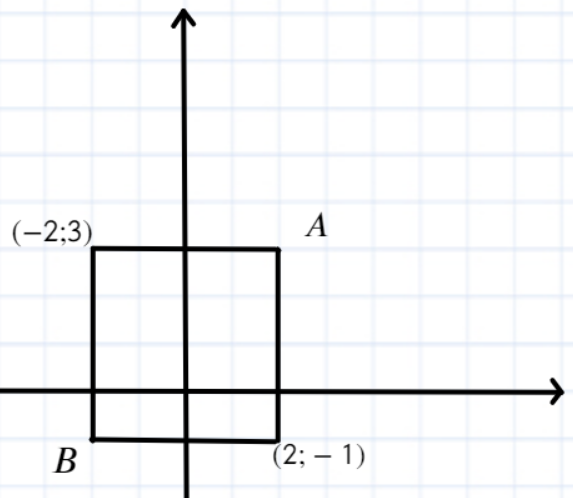
\includegraphics[width=1\linewidth]{kv1.png}
 %% метка рисунка для ссылки на него
\end{minipage}
\hfill
\begin{minipage}[h]{0.4\linewidth}
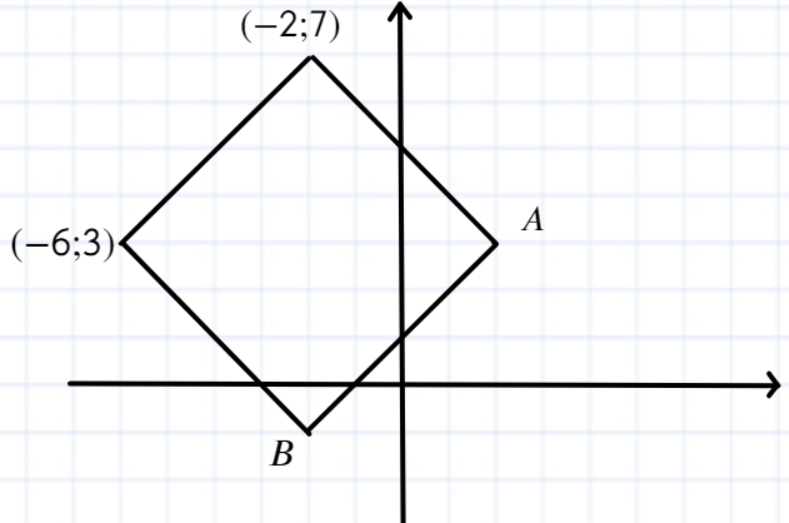
\includegraphics[width=1\linewidth]{kv2.png}
\end{minipage}
\hfill
\begin{minipage}[h]{0.2\linewidth}
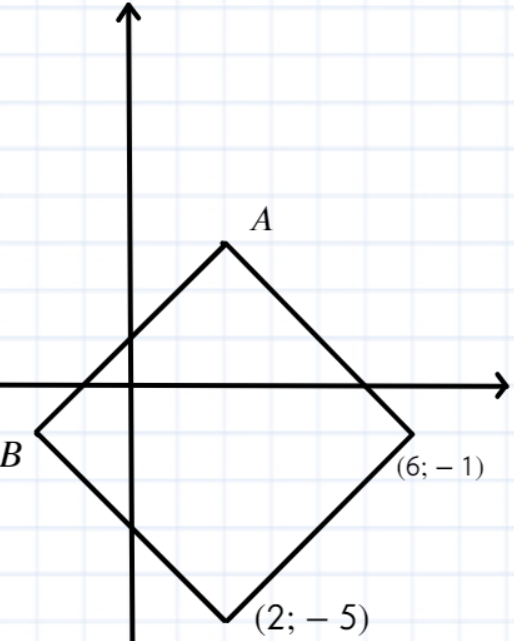
\includegraphics[width=1\linewidth]{kv3.png}
 %% метка рисунка для ссылки на него
\end{minipage}
\hfill
\end{center}
\end{figure}\\
